\documentclass[11pt]{article}
\usepackage[UTF8]{ctex}
\usepackage{subcaption}
%%%%%%%%%%%%%%%%%%%%%%%%%%%%%%%%%%%%%%%%%
% Cleese Assignment
% Structure Specification File
% Version 1.0 (27/5/2018)
%
% This template originates from:
% http://www.LaTeXTemplates.com
%
% Author:
% Vel (vel@LaTeXTemplates.com)
%
% License:
% CC BY-NC-SA 3.0 (http://creativecommons.org/licenses/by-nc-sa/3.0/)
%
%%%%%%%%%%%%%%%%%%%%%%%%%%%%%%%%%%%%%%%%%

%----------------------------------------------------------------------------------------
%	PACKAGES AND OTHER DOCUMENT CONFIGURATIONS
%----------------------------------------------------------------------------------------

\usepackage{lastpage} % Required to determine the last page number for the footer

\usepackage{graphicx} % Required to insert images

\setlength\parindent{0pt} % Removes all indentation from paragraphs

\usepackage[most]{tcolorbox} % Required for boxes that split across pages

\usepackage{booktabs} % Required for better horizontal rules in tables

\usepackage{listings} % Required for insertion of code

\usepackage{etoolbox} % Required for if statements

\usepackage{amsmath}
\usepackage{amsthm}
\usepackage{amssymb}
\usepackage{indentfirst}
\usepackage{diagbox}
\usepackage{subfigure}
\usepackage{float}
\usepackage{xcolor}
\usepackage[colorlinks, linkcolor = black]{hyperref}

\usepackage{enumerate}
\usepackage{enumitem}
\setlist{
    leftmargin = .1\linewidth,
    % rightmargin = .1\linewidth,
    % label=\emph{\alph*}.
}

\setlength{\parindent}{2em}

\usepackage{siunitx}
\sisetup
{
    output-exponent-marker = \ensuremath{\mathrm{E}},
    exponent-product = {},
    retain-explicit-plus,
    retain-zero-exponent,
}
%----------------------------------------------------------------------------------------
%	MARGINS
%----------------------------------------------------------------------------------------

\usepackage{geometry} % Required for adjusting page dimensions and margins

\geometry{
    paper=a4paper, % Change to letterpaper for US letter
    top=3cm, % Top margin
    bottom=3cm, % Bottom margin
    left=2.5cm, % Left margin
    right=2.5cm, % Right margin
    headheight=14pt, % Header height
    footskip=1.4cm, % Space from the bottom margin to the baseline of the footer
    headsep=1.2cm, % Space from the top margin to the baseline of the header
    %showframe, % Uncomment to show how the type block is set on the page
}

%----------------------------------------------------------------------------------------
%	FONT
%----------------------------------------------------------------------------------------

\usepackage[utf8]{inputenc} % Required for inputting international characters
\usepackage[T1]{fontenc} % Output font encoding for international characters

% \usepackage[sfdefault,light]{roboto} % Use the Roboto font

%----------------------------------------------------------------------------------------
%	HEADERS AND FOOTERS
%----------------------------------------------------------------------------------------

\usepackage{fancyhdr} % Required for customising headers and footers

\pagestyle{fancy} % Enable custom headers and footers

\lhead{\small\assignmentClass} % Left header; output the instructor in brackets if one was set
\chead{\small\assignmentTitle} % Centre header
\rhead{\small\ifdef{\assignmentAuthorName}{\assignmentAuthorName}{\ifdef{\assignmentDate}{Due\ \assignmentDate}{}}} % Right header; output the author name if one was set, otherwise the due date if that was set

\lfoot{} % Left footer
\cfoot{\small Page\ \thepage\ of\ \pageref{LastPage}} % Centre footer
\rfoot{} % Right footer

\renewcommand\headrulewidth{0.5pt} % Thickness of the header rule

%----------------------------------------------------------------------------------------
%	MODIFY SECTION STYLES
%----------------------------------------------------------------------------------------

\usepackage{titlesec} % Required for modifying sections

%------------------------------------------------
% Section

\titleformat
{\section} % Section type being modified
[block] % Shape type, can be: hang, block, display, runin, leftmargin, rightmargin, drop, wrap, frame
{\Large\bfseries} % Format of the whole section
{\arabic{section}} % Format of the section label
{6pt} % Space between the title and label
{} % Code before the label

\titlespacing{\section}{0pt}{0.5\baselineskip}{0.5\baselineskip} % Spacing around section titles, the order is: left, before and after

%------------------------------------------------
% Subsection

\titleformat
{\subsection} % Section type being modified
[block] % Shape type, can be: hang, block, display, runin, leftmargin, rightmargin, drop, wrap, frame
{\itshape} % Format of the whole section
{(\arabic{subsection})} % Format of the section label
{4pt} % Space between the title and label
{} % Code before the label

\titlespacing{\subsection}{0pt}{0.5\baselineskip}{0.5\baselineskip} % Spacing around section titles, the order is: left, before and after

\renewcommand\thesubsection{(\arabic{subsection})}

%----------------------------------------------------------------------------------------
%	CUSTOM QUESTION COMMANDS/ENVIRONMENTS
%----------------------------------------------------------------------------------------



% Command to print an assignment section title to split an assignment into major parts
\newcommand{\assignmentSection}[1]{
    \newpage
    {
        \centering % Centre the section title
        \vspace{2\baselineskip} % Whitespace before the entire section title

        \rule{0.8\textwidth}{0.5pt} % Horizontal rule

        \vspace{0.75\baselineskip} % Whitespace before the section title
        {\LARGE \textsc{#1}} % Section title, forced to be uppercase

        \rule{0.8\textwidth}{0.5pt} % Horizontal rule

        \vspace{\baselineskip} % Whitespace after the entire section title
    }
    \setcounter{section}{0}

}

%----------------------------------------------------------------------------------------
%	TITLE PAGE
%----------------------------------------------------------------------------------------

\author{\textbf{\assignmentNo\ \assignmentAuthorName}} % Set the default title page author field
\date{} % Don't use the default title page date field

\title{
    \thispagestyle{empty} % Suppress headers and footers
    \vspace{0.2\textheight} % Whitespace before the title
    \textbf{\assignmentClass}\\[5pt]
    \texttt{\assignmentTitle}\\[-4pt]
    % \ifdef{\assignmentSubTitle}{\texttt{\assignmentSubTitle}}{}
    \ifdef{\assignmentDate}{\assignmentDate}{} % If a due date is supplied, output it
    \ifdef{\assignmentClassInstructor}{{\large \textit{\assignmentClassInstructor}}}{} % If an instructor is supplied, output it
    \vspace{0.32\textheight} % Whitespace before the author name
}

\newtheorem{Theorem}{定理}
\newtheorem{Lemma}{引理}
\newtheorem{Proof}{证明}

\sisetup
{
    table-format = +1.12e+003,
}

\newcommand{\assignmentQuestionName}{Question} % The word to be used as a prefix to question numbers; example alternatives: Problem, Exercise
\newcommand{\assignmentClass}{计算方法B} % Course/class
\newcommand{\assignmentTitle}{Programming Assignment\ \#3}
\newcommand{\assignmentDate}{2020.4.25} % date
\newcommand{\assignmentNo}{PB17000297}
\newcommand{\assignmentAuthorName}{罗晏宸} % Student name

\begin{document}

\maketitle % Print the title page

\thispagestyle{empty} % Suppress headers and footers on the title page

\newpage

\assignmentSection{非线性方程求根}
\section{问题描述}
分别编写用 Newton 法和弦截法求根的通用程序。再利用你的通用程序分别求下面方程的根
$$
    f(x) = 2x^4 + 24x^3 + 61x - 16x + 1 = 0
$$
其中, Newton 迭代法分别取初值 $x_0 = 0$ 和 $x_0 = 3$;弦截法的初值分别取为 $x_0 = 0,\ x_1 = 0.5$ 以及 $x_0 = 0.1,\ x_1 = 1.5$;

取误差限$\varepsilon$为\num{1.0e-9},即当$|f(x_k)| < \varepsilon$时,停止迭代。将计算结果列成表格,要求给出初值、每步的迭代结果,以及最终的迭代结果(包括迭代步数);比较或分析两种计算方法的优劣。

\section{计算结果}
由 C++ 计算得到结果按格式输出并列表如下,数据由 Mathematica 绘图,迭代过程中 Newton 法所有的切线与弦截法所有的弦均已绘出,但考虑视觉可辨识度,仅对迭代开始时的几个 $x$ 轴交点做了标注。

\begin{figure}[h]
    \centering
    \begin{subfigure}{.49\textwidth}
        \centering
        \scalebox{0.75}{
            \begin{tabular}{|l|c|c|}
                \hline
                迭代步数$k$            & $x_k$                        & $f(x_k)$                     \\
                \hline $k = 0$(初值) & $0.0000000000\text{E}{+}000$ & $1.0000000000\text{E}{+}000$ \\
                \hline $k = 1$         & $6.2500000000\text{E}{-}002$ & $2.4417114258\text{E}{-}001$ \\
                \hline $k = 2$         & $9.2675144823\text{E}{-}002$ & $6.0357821710\text{E}{-}002$ \\
                \hline $k = 3$         & $1.0750916023\text{E}{-}001$ & $1.4994760152\text{E}{-}002$ \\
                \hline $k = 4$         & $1.1485323376\text{E}{-}001$ & $3.7248898748\text{E}{-}003$ \\
                \hline $k = 5$         & $1.1848368152\text{E}{-}001$ & $9.1626064336\text{E}{-}004$ \\
                \hline $k = 6$         & $1.2024260677\text{E}{-}001$ & $2.1577268802\text{E}{-}004$ \\
                \hline $k = 7$         & $1.2102581790\text{E}{-}001$ & $4.2847681852\text{E}{-}005$ \\
                \hline $k = 8$         & $1.2128383271\text{E}{-}001$ & $4.6530959359\text{E}{-}006$ \\
                \hline $k = 9$         & $1.2131962667\text{E}{-}001$ & $8.9569062833\text{E}{-}008$ \\
                \hline $k = 10$        & $1.2132034327\text{E}{-}001$ & $3.5900726836\text{E}{-}011$ \\
                \hline \multicolumn{3}{|c|}{$|f(x_{10})| < \varepsilon$,停止迭代}                   \\
                \hline
            \end{tabular}
        }
        \label{table:Newton1}
    \end{subfigure}
    \begin{subfigure}{.49\textwidth}
        \centering
        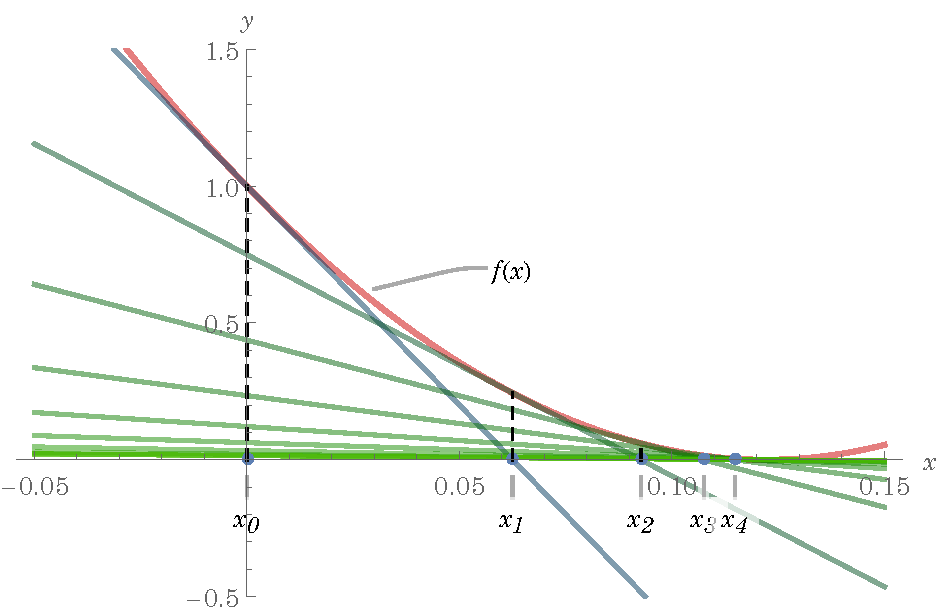
\includegraphics[scale = 0.5]{Figure/Newton1.pdf}
        \label{figure:Newton1}
    \end{subfigure}
    \caption{Newton 法迭代结果 1 }
    \label{Newton1}
\end{figure}
\begin{figure}
    \centering
    \begin{subfigure}{.49\textwidth}
        \centering
        \scalebox{0.75}{
            \begin{tabular}{|l|c|c|}
                \hline
                迭代步数$k$            & $x_k$                        & $f(x_k)$                     \\
                \hline $k = 0$(初值) & $3.0000000000\text{E}{+}000$ & $1.3120000000\text{E}{+}003$ \\
                \hline $k = 1$         & $1.9192751236\text{E}{+}000$ & $3.9180729077\text{E}{+}002$ \\
                \hline $k = 2$         & $1.1936133228\text{E}{+}000$ & $1.1368262566\text{E}{+}002$ \\
                \hline $k = 3$         & $7.3112145458\text{E}{-}001$ & $3.1859876182\text{E}{+}001$ \\
                \hline $k = 4$         & $4.5362080609\text{E}{-}001$ & $8.6190504416\text{E}{+}000$ \\
                \hline $k = 5$         & $2.9663693142\text{E}{-}001$ & $2.2633471161\text{E}{+}000$ \\
                \hline $k = 6$         & $2.1197535112\text{E}{-}001$ & $5.8197426653\text{E}{-}001$ \\
                \hline $k = 7$         & $1.6779403531\text{E}{-}001$ & $1.4770709460\text{E}{-}001$ \\
                \hline $k = 8$         & $1.4519438879\text{E}{-}001$ & $3.7206334228\text{E}{-}002$ \\
                \hline $k = 9$         & $1.3376760731\text{E}{-}001$ & $9.3253679860\text{E}{-}003$ \\
                \hline $k = 10$        & $1.2803649704\text{E}{-}001$ & $2.3222638207\text{E}{-}003$ \\
                \hline $k = 11$        & $1.2519603327\text{E}{-}001$ & $5.6755417123\text{E}{-}004$ \\
                \hline $k = 12$        & $1.2383872242\text{E}{-}001$ & $1.2927049695\text{E}{-}004$ \\
                \hline $k = 13$        & $1.2327102895\text{E}{-}001$ & $2.2587102744\text{E}{-}005$ \\
                \hline $k = 14$        & $1.2311856261\text{E}{-}001$ & $1.6284754711\text{E}{-}006$ \\
                \hline $k = 15$        & $1.2310571808\text{E}{-}001$ & $1.1556329893\text{E}{-}008$ \\
                \hline $k = 16$        & $1.2310562562\text{E}{-}001$ & $5.9885429948\text{E}{-}013$ \\
                \hline \multicolumn{3}{|c|}{$|f(x_{16})| < \varepsilon$,停止迭代}                   \\
                \hline
            \end{tabular}
        }
        \label{table:Newton2}
    \end{subfigure}
    \begin{subfigure}{.49\textwidth}
        \centering
        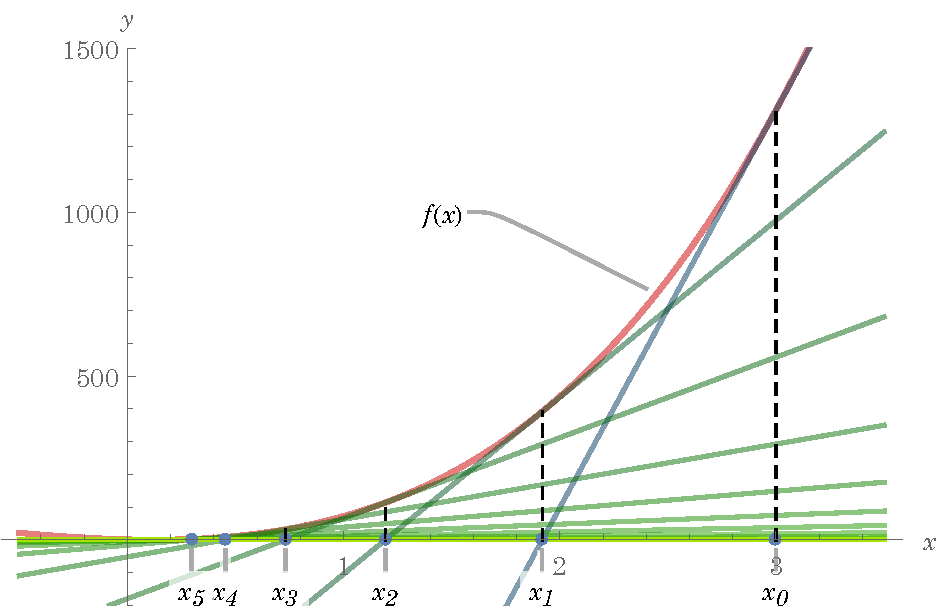
\includegraphics[scale = 0.5]{Figure/Newton2.pdf}
        \label{figure:Newton2}
    \end{subfigure}
    \caption{Newton 法迭代结果 2 }
    \label{Newton2}
\end{figure}
\begin{figure}
    \centering
    \begin{subfigure}{.49\textwidth}
        \centering
        \scalebox{0.75}{
            \begin{tabular}{|l|c|c|}
                \hline
                迭代步数$k$            & $x_k$                         & $f(x_k)$                     \\
                \hline $k = 0$(初值) & $+0.0000000000\text{E}{+}000$ & $1.0000000000\text{E}{+}000$ \\
                \hline $k = 1$(初值) & $+5.0000000000\text{E}{-}001$ & $1.1375000000\text{E}{+}001$ \\
                \hline $k = 2$         & $-4.8192771084\text{E}{-}002$ & $1.9100839450\text{E}{+}000$ \\
                \hline $k = 3$         & $-1.5882177241\text{E}{-}001$ & $4.9849583298\text{E}{+}000$ \\
                \hline $k = 4$         & $+2.0528956326\text{E}{-}002$ & $6.9745241532\text{E}{-}001$ \\
                \hline $k = 5$         & $+4.9704099508\text{E}{-}002$ & $3.5839401507\text{E}{-}001$ \\
                \hline $k = 6$         & $+8.0543024888\text{E}{-}002$ & $1.1965360731\text{E}{-}001$ \\
                \hline $k = 7$         & $+9.5999095782\text{E}{-}002$ & $4.7582804260\text{E}{-}002$ \\
                \hline $k = 8$         & $+1.0620354980\text{E}{-}001$ & $1.7777847602\text{E}{-}002$ \\
                \hline $k = 9$         & $+1.1229022963\text{E}{-}001$ & $6.8102183582\text{E}{-}003$ \\
                \hline $k = 10$        & $+1.1606968076\text{E}{-}001$ & $2.5795784215\text{E}{-}003$ \\
                \hline $k = 11$        & $+1.1837415259\text{E}{-}001$ & $9.7415265691\text{E}{-}004$ \\
                \hline $k = 12$        & $+1.1977247782\text{E}{-}001$ & $3.6072356011\text{E}{-}004$ \\
                \hline $k = 13$        & $+1.2059475518\text{E}{-}001$ & $1.2741741436\text{E}{-}004$ \\
                \hline $k = 14$        & $+1.2104383231\text{E}{-}001$ & $3.9878767168\text{E}{-}005$ \\
                \hline $k = 15$        & $+1.2124841215\text{E}{-}001$ & $9.3453570276\text{E}{-}006$ \\
                \hline $k = 16$        & $+1.2131102788\text{E}{-}001$ & $1.1695181286\text{E}{-}006$ \\
                \hline $k = 17$        & $+1.2131998479\text{E}{-}001$ & $4.4816937383\text{E}{-}008$ \\
                \hline $k = 18$        & $+1.2132034170\text{E}{-}001$ & $2.3240176450\text{E}{-}010$ \\
                \hline \multicolumn{3}{|c|}{$|f(x_{18})| < \varepsilon$,停止迭代}                    \\
                \hline
            \end{tabular}
        }
        \label{table:Secant1}
    \end{subfigure}
    \begin{subfigure}{.49\textwidth}
        \centering
        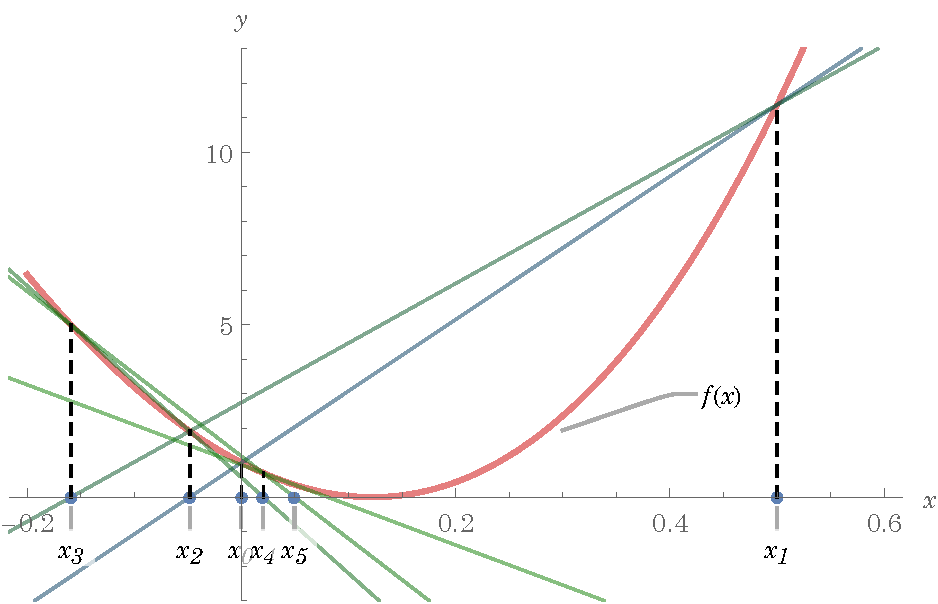
\includegraphics[scale = 0.45]{Figure/Secant1.pdf}
        \label{figure:Secant1}
    \end{subfigure}
    \caption{弦截法迭代结果 1 }
    \label{Secant1}
\end{figure}
\begin{figure}
    \centering
    \begin{subfigure}{.65\textwidth}
        \centering
        \begin{tabular}{|l|c|c|}
            \hline
            迭代步数$k$            & $x_k$                        & $f(x_k)$                     \\
            \hline $k = 0$(初值) & $1.0000000000\text{E}{-}001$ & $3.4200000000\text{E}{-}002$ \\
            \hline $k = 1$(初值) & $1.5000000000\text{E}{+}000$ & $2.0537500000\text{E}{+}002$ \\
            \hline $k = 2$         & $9.9766826661\text{E}{-}002$ & $3.4920022729\text{E}{-}002$ \\
            \hline $k = 3$         & $9.9528703766\text{E}{-}002$ & $3.5662994682\text{E}{-}002$ \\
            \hline $k = 4$         & $1.1095871197\text{E}{-}001$ & $8.7722830757\text{E}{-}003$ \\
            \hline $k = 5$         & $1.1468740718\text{E}{-}001$ & $3.8969392942\text{E}{-}003$ \\
            \hline $k = 6$         & $1.1766781216\text{E}{-}001$ & $1.3876451955\text{E}{-}003$ \\
            \hline $k = 7$         & $1.1931598272\text{E}{-}001$ & $5.3099453171\text{E}{-}004$ \\
            \hline $k = 8$         & $1.2033760050\text{E}{-}001$ & $1.9023231922\text{E}{-}004$ \\
            \hline $k = 9$         & $1.2090792407\text{E}{-}001$ & $6.3397280115\text{E}{-}005$ \\
            \hline $k = 10$        & $1.2119299484\text{E}{-}001$ & $1.7038550552\text{E}{-}005$ \\
            \hline $k = 11$        & $1.2129776891\text{E}{-}001$ & $2.8550135170\text{E}{-}006$ \\
            \hline $k = 12$        & $1.2131885895\text{E}{-}001$ & $1.8556909953\text{E}{-}007$ \\
            \hline $k = 13$        & $1.2132032505\text{E}{-}001$ & $2.3119210990\text{E}{-}009$ \\
            \hline $k = 14$        & $1.2132034354\text{E}{-}001$ & $1.9196866319\text{E}{-}012$ \\
            \hline \multicolumn{3}{|c|}{$|f(x_{14})| < \varepsilon$,停止迭代}                   \\
            \hline
        \end{tabular}
        \label{table:Secant2}
    \end{subfigure}
    \begin{subfigure}{.33\textwidth}
        \centering
        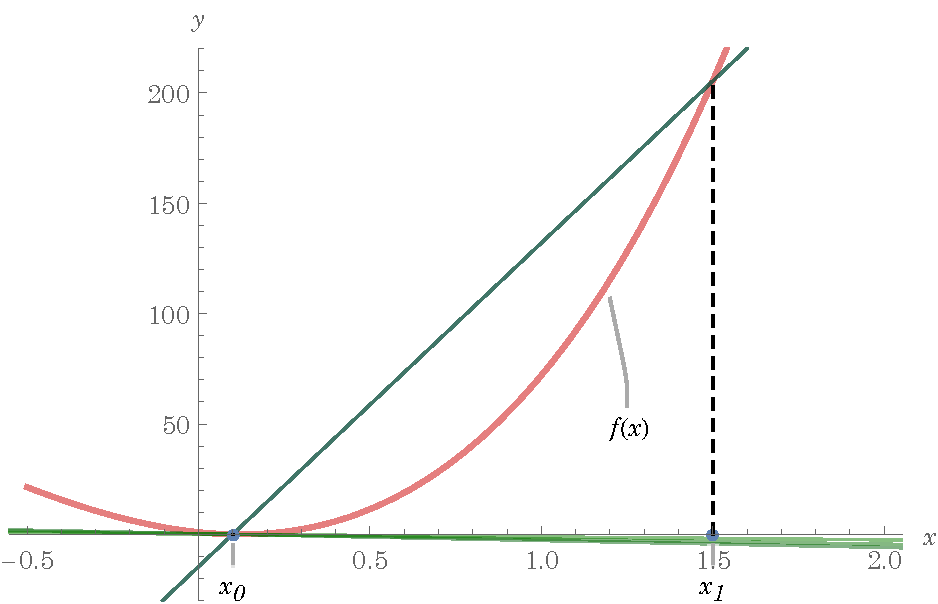
\includegraphics[scale = 0.33]{Figure/Secant2.pdf}
        \caption{整体示意图}
        \label{figure:Secant2}
    \end{subfigure}
    \begin{subfigure}{\textwidth}
        \centering
        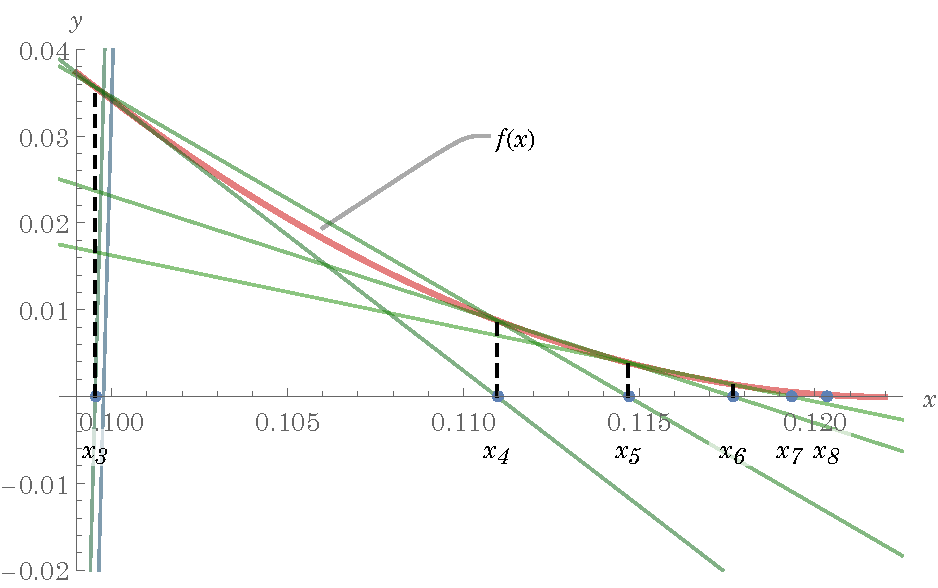
\includegraphics[scale = 0.8]{Figure/Secant2-zoom.pdf}
        \caption{局部放大图}
        \label{figure:Secant2-zoom}
    \end{subfigure}
    \caption{弦截法迭代结果 2 }
    \label{Secant2}
\end{figure}

\section{结果分析}
由不同初值两种方法分别得到的迭代结果可知,函数$f(x) = 2x^4 + 24x^3 + 61x - 16x + 1$有数值值在$0.1213$和(或)$0.1231$附近的根。代数计算得到方程$f(x) = 0$在这附近有两个解
$$
    \alpha = \frac{3 \sqrt{2} - 4}{2},\ \beta = \sqrt{17} - 4
$$
对比计算结果,除了初值为$x_0 = 3$的 Newton 法迭代在误差限内向$\beta$收敛,其他三组结果均向$\alpha$收敛。结合图像可知,函数在$0.1222$附近有一驻点$\gamma \in (\alpha, \beta)$,对于 Newton 法而言,初始值$x_0 = 0$与$x_0 = 3$分别在$\alpha$左侧导数为负以及$\beta$右侧导数为正处,因此分别向两者收敛。对于弦截法而言,由于第一次迭代实际上是求得过$(x_0,\, f(x_0))$和$(x_1,\, f(x_1))$两点直线和$x$的交点,对于两组不同初值的弦截法迭代过程,由于$x_1$相比$x_0$较为远离驻点$\gamma$,即$f(x_1)$相比$f(x_0)$及$f(x_2)$均较大,所以前两次计算得到的迭代点$x_2$和$x_3$均落在$\alpha$左侧导数为负处,随后的迭代过程随即向$\alpha$收敛。

以不同初值进行的迭代,步数$k$有所差异:初值为$x_0 = 0$和$x_0 = 3$的 Newton 法迭代步数分别为 10 次和 16 次,初值为$x_0 = 0,\ x_1 = 0.5$和$x_0 = 0.1,\ x_1 = 1.5$的弦截法迭代步数分别为 18 次和 14 次。

注意到$x_0 = 0$较$x_0 = 3$更接近相应迭代序列所收敛的函数的根,同时受收敛方向上函数导数的影响,以前者为初值的 Newton 法迭代在$k = 2$时即已将迭代结果对应的函数值控制在\num{1E-1}以内,而后者在$k = 8$时才控制到相当的量级。在相同的误差限条件下,前者总的迭代步数也较后者少。对于弦截法,两组初值均存在$x_0$在根左侧$x_1$在根右侧的结构,从图像上也可以看到前两次迭代对应的截线均比较明显且有较大的正斜率,同时均从$x_3$开始迭代点向根保持正增量。但注意到初值为$x_0 = 0,\ x_1 = 0.5$的弦截法迭代过程中$x_2$与$x_3$都落到了$x$轴负半轴$f(x)$斜率绝对值较大处,相比之下初值为$x_0 = 0.1,\ x_1 = 1.5$的弦截法迭代过程中从$x_2$开始迭代点对应$f(x)$的倾斜程度较小,能够更快地收敛。

在之后的算法分析部分,将会对两种方法四组迭代过程速度做定量的分析。

\section{算法分析}
\subsection{理论收敛性}
对于Newton 迭代法,在$f(x)$的零点$\alpha = \frac{3 \sqrt{2} - 4}{2}$和$\beta = \sqrt{17} - 4处$,有
\begin{align*}
    |\varphi'(\alpha)| & = \left.\left|\frac{f(x)f''(x)}{\left(f'(x)\right)^2}\right|\right|_{x = \alpha} \\
                       & = 0                                                                              \\
    |\varphi'(\beta)|  & =0
\end{align*}
且
\begin{align*}
    |\varphi'(0)| & = \left.\left|\frac{f(x)f''(x)}{\left(f'(x)\right)^2}\right|\right|_{x = 0}                                                                  \\
                  & = \left.\frac{48 x^6+864 x^5+5164 x^4+11328 x^3+5162 x^2-1808 x+122}{64 x^6+1152 x^5+7136 x^4+17312 x^3+12580 x^2-3904 x+256}\right|_{x = 0} \\
                  & = \frac{61}{128}                                                                                                                             \\
                  & \approx 0.476563 < 1
                  &                                                                                                                                              \\
    |\varphi'(3)| & = \frac{252560}{368449}                                                                                                                      \\
                  & \approx 0.685468 < 1
\end{align*}
因此理论上初值为$x_0 = 0$ 和$x_0 = 3$的 Newton 迭代都是收敛的。

对于弦截法的收敛判断可由如下定理给出\cite{2005数值分析}:
\begin{Theorem}
    若 $f(x)$ 在根$x^*$的某个邻域$U(x^*,\, \delta)$内有二阶连续导数,且对任意的$x \in U(x^*,\, \delta)$有$f'(x) \neq 0$,则当$\delta$充分小时,对$U(x^*,\, \delta)$内任意的$x_0$和$x_1$,弦截法迭代公式
    \begin{equation}
        x_{k + 1} = x_k - \frac{f(x_k)(x_k - x_{k - 1})}{f(x_k) - f(x_{k - 1})} \label{1} \tag{1}
    \end{equation}
    得到的迭代序列$\{x_n\}$收敛到方程 $f(x) = 0$ 的根$x^*$。
\end{Theorem}
\begin{proof}
    首先用归纳法证明,当$x_{n - 1}, x_n \in U(x^*,\, \delta)$时,$x_{n + 1} \in U(x^*,\, \delta)$。
    过点$(x_{n - 1}, f(x_{n - 1}))$和$(x_{n}, f(x_{n}))$的直线方程为
    \begin{equation*}
        l_1(x) = f(x_{n - 1}) + \frac{f(x_n) - f(x_{n - 1})}{x_n - x_{n - 1}}(x - x_{n - 1})
    \end{equation*}
    则有线性插值余项
    \begin{equation*}
        f(x) - l_1(x) = \frac{1}{2}f'(\xi_1)(x^* - x_{n - 1})
    \end{equation*}
    由于 $f(x^*) = 0$,有
    \begin{align*}
        l_1(x^*) & = -\frac{1}{2} f'(\xi_1)(x^* - x_n)(x^* - x_{n - 1})  \\
                 & = -\frac{1}{2}f'(\xi_1)e_ne_{n - 1} \label{2} \tag{2}
    \end{align*}
    其中$e_n = x_n - x^*$表示迭代误差。

    另一方面,由弦截法知$x_{n + 1}$是方程$l_1(x) = 0$的根,所以
    \begin{align*}
        l_1(x^*) & = l_1(x^*) - l_1(x_{n + 1})                                      \\
                 & = \frac{f(x_n) - f(x_{n - 1})}{x_n - x_{n - 1}}(x^* - x_{n + 1}) \\
                 & = -f'(\xi_2)(x_{n + 1} - x^*)                                    \\
                 & = -f'(\xi_2)e_{n + 1} \label{3} \tag{3}
    \end{align*}
    由式\eqref{2}和\eqref{3}得
    \begin{equation}
        e_{n + 1} = \frac{f'(\xi_1)}{2f'(\xi_2)}e_ne_{n - 1} \label{4} \tag{4}
    \end{equation}
    因为$\xi_1$和$\xi_2$均在$x_{n - 1}$、$x_n$和$x^*$所确定的区间内,所以当$x_{n - 1}, x_n \in U(x^*,\, \delta)$时,有$\xi_1, \xi_2 \in U(x^*,\, \delta)$。令
    \begin{equation*}
        M = \frac{\displaystyle \max_{x \in U(x^*,\, \delta)}{\left|f'(x)\right|}}{\displaystyle \min_{x \in U(x^*,\, \delta)}{\left|f'(x)\right|}}
    \end{equation*}
    选取邻域$U(x^*,\, \delta)$充分小,使得$M\delta < 1$,则当$x_{n - 1}, x_n \in U(x^*,\, \delta)$时,由式\eqref{4}有
    \begin{align*}
        \left|e_{n + 1}\right| & \leqslant \frac{1}{2}M\left|e_{n}\right|\left|e_{n - 1}\right| \\
                               & \leqslant \frac{1}{2}M\delta                                   \\
                               & < \delta \label{5} \tag{5}
    \end{align*}
    于是 $x_{n + 1} \in U(x^*,\, \delta)$。由假定$x_0, x_1 \in U(x^*,\, \delta)$,从而$\forall n,\ x_n \in U(x^*,\, \delta)$。

    其次,由式\eqref{5}知
    \begin{equation*}
        \left|e_{n}\right| \leqslant \frac{1}{M}(M\delta)^n
    \end{equation*}
    故有$\displaystyle \lim_{n \rightarrow \infty}{\left|e_{n}\right|} = 0$,即$\displaystyle \lim_{n \rightarrow \infty}{x_n} = x^*$,因此迭代收敛。
\end{proof}
由于多项式函数$f(x)$在数轴上是无穷光滑的,且由前述讨论可知,在$x > 0$范围内$f(x)$的唯一驻点$\gamma$不在迭代进行的区间内,因此理论上初值为$x_0 = 0,\ x_1 = 0.5$和$x_0 = 0.1,\ x_1 = 1.5$的弦截法迭代也都是收敛的

\subsection{收敛阶}
由于$\alpha$和$\beta$均为$f(x)$的单根,因此采用的 Newton 迭代方程
\begin{equation}
    x_{k + 1} = \varphi(x_k) = x_k - \frac{f(x_k)}{f'(x_k)} \label{6} \tag{6}
\end{equation}
理论上是 2 阶迭代方法。为根据实验数据对此进行验证,由收敛阶$n$的定义式
\begin{equation*}
    \lim_{k \rightarrow \infty}{\frac{\left|e_{k + 1}\right|}{\left|e_{k}\right|^n}} = \lim_{k \rightarrow \infty}{\frac{\left|x_{k + 1} - \alpha \right|}{\left|x_k - \alpha \right|^n}} = M
\end{equation*}
对$\{(\ln{e_{k}},\, \ln{e_{k + 1}})\},\ k = 0,\, 1,\, \cdots$做最小二乘拟合,则直线斜率以收敛阶$n$为极限\cite{数值方法计算弦截法的收敛阶}。为了在$k$充分大的条件下验证收敛阶,我们选取每组迭代序列最后 5 个数值点进行拟合,拟合结果如图\ref{Newton-LS1}和\ref{Newton-LS2}所示。
\begin{figure}[h]
    \centering
    \begin{subfigure}{\textwidth}
        \centering
        \resizebox{\textwidth}{!}{
            \begin{tabular}{|c|c|c|c|c|}
                \hline
                迭代步数$k$     & $x_k$                        & $e_k$                        & $\ln{e_{k}}$                  & $\ln{e_{k + 1}}$              \\
                \hline $k = 0$  & $0.0000000000\text{E}{+}000$ & $1.2132034356\text{E}{-}001$ & $-2.1093207643\text{E}{+}000$ & $-2.8332675050\text{E}{+}000$ \\
                \hline $k = 1$  & $6.2500000000\text{E}{-}002$ & $5.8820343560\text{E}{-}002$ & $-2.8332675050\text{E}{+}000$ & $-3.5527694332\text{E}{+}000$ \\
                \hline $k = 2$  & $9.2675144823\text{E}{-}002$ & $2.8645198737\text{E}{-}002$ & $-3.5527694332\text{E}{+}000$ & $-4.2822766288\text{E}{+}000$ \\
                \hline $k = 3$  & $1.0750916023\text{E}{-}001$ & $1.3811183330\text{E}{-}002$ & $-4.2822766288\text{E}{+}000$ & $-5.0410259787\text{E}{+}000$ \\
                \hline $k = 4$  & $1.1485323376\text{E}{-}001$ & $6.4671097966\text{E}{-}003$ & $-5.0410259787\text{E}{+}000$ & $-5.8651272568\text{E}{+}000$ \\
                \hline $k = 5$  & $1.1848368152\text{E}{-}001$ & $2.8366620379\text{E}{-}003$ & $-5.8651272568\text{E}{+}000$ & $-6.8328920059\text{E}{+}000$ \\
                \hline $k = 6$  & $1.2024260677\text{E}{-}001$ & $1.0777367852\text{E}{-}003$ & $-6.8328920059\text{E}{+}000$ & $-8.1301444249\text{E}{+}000$ \\
                \hline $k = 7$  & $1.2102581790\text{E}{-}001$ & $2.9452566089\text{E}{-}004$ & $-8.1301444249\text{E}{+}000$ & $-1.0217900978\text{E}{+}001$ \\
                \hline $k = 8$  & $1.2128383271\text{E}{-}001$ & $3.6510853775\text{E}{-}005$ & $-1.0217900978\text{E}{+}001$ & $-1.4148348605\text{E}{+}001$ \\
                \hline $k = 9$  & $1.2131962667\text{E}{-}001$ & $7.1688628629\text{E}{-}007$ & $-1.4148348605\text{E}{+}001$ & $-2.1969957865\text{E}{+}001$ \\
                \hline $k = 10$ & $1.2132034327\text{E}{-}001$ & $2.8745411607\text{E}{-}010$ & $-2.1969957865\text{E}{+}001$ &                               \\
                \hline
            \end{tabular}
        }
        \label{table:Newton-LS1}
    \end{subfigure}
    \begin{subfigure}{.49\textwidth}
        \centering
        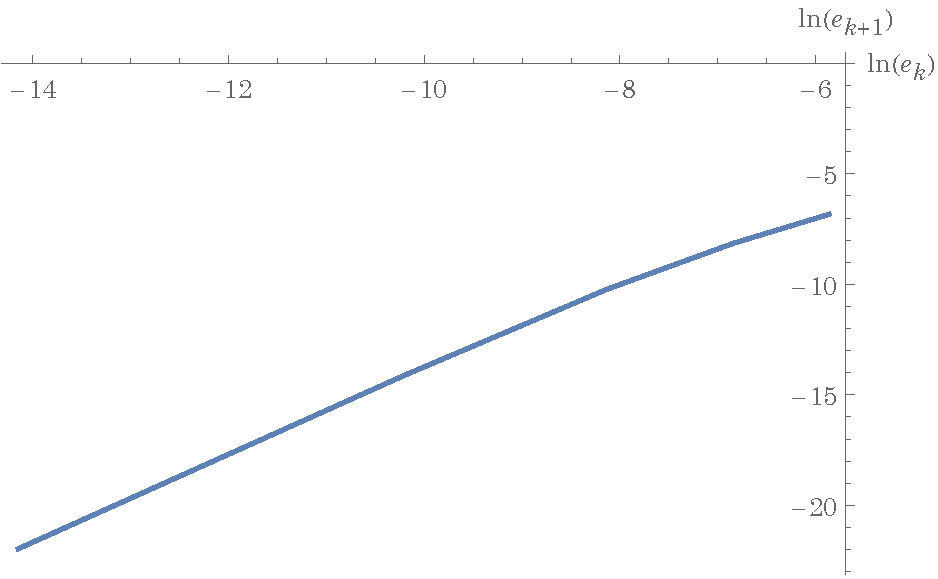
\includegraphics[scale = 0.5]{Figure/收敛阶-Newton1.pdf}
        \label{figure:Newton-LS1}
    \end{subfigure}
    \begin{subfigure}{.49\textwidth}
        \centering
        拟合直线方程为
        \begin{equation*}
            1.8499 x + 4.46115
        \end{equation*}
    \end{subfigure}
    \caption{最小二乘拟合Newton 法结果 1 收敛阶}
    \label{Newton-LS1}
\end{figure}
\begin{figure}[h]
    \centering
    \begin{subfigure}{\textwidth}
        \centering
        \resizebox{\textwidth}{!}{
            \begin{tabular}{|c|c|c|c|c|}
                \hline
                迭代步数$k$     & $x_k$                        & $e_k$                        & $\ln{e_{k}}$                  & $\ln{e_{k + 1}}$              \\
                \hline $k = 0$  & $3.0000000000\text{E}{+}000$ & $2.8768943744\text{E}{+}000$ & $+1.0567113701\text{E}{+}000$ & $+5.8565634067\text{E}{-}001$ \\
                \hline $k = 1$  & $1.9192751236\text{E}{+}000$ & $1.7961694979\text{E}{+}000$ & $+5.8565634067\text{E}{-}001$ & $+6.8133019265\text{E}{-}002$ \\
                \hline $k = 2$  & $1.1936133228\text{E}{+}000$ & $1.0705076972\text{E}{+}000$ & $+6.8133019265\text{E}{-}002$ & $-4.9755436287\text{E}{-}001$ \\
                \hline $k = 3$  & $7.3112145458\text{E}{-}001$ & $6.0801582897\text{E}{-}001$ & $-4.9755436287\text{E}{-}001$ & $-1.1071026889\text{E}{+}000$ \\
                \hline $k = 4$  & $4.5362080609\text{E}{-}001$ & $3.3051518047\text{E}{-}001$ & $-1.1071026889\text{E}{+}000$ & $-1.7513972590\text{E}{+}000$ \\
                \hline $k = 5$  & $2.9663693142\text{E}{-}001$ & $1.7353130580\text{E}{-}001$ & $-1.7513972590\text{E}{+}000$ & $-2.4205837400\text{E}{+}000$ \\
                \hline $k = 6$  & $2.1197535112\text{E}{-}001$ & $8.8869725502\text{E}{-}002$ & $-2.4205837400\text{E}{+}000$ & $-3.1080411020\text{E}{+}000$ \\
                \hline $k = 7$  & $1.6779403531\text{E}{-}001$ & $4.4688409691\text{E}{-}002$ & $-3.1080411020\text{E}{+}000$ & $-3.8126862535\text{E}{+}000$ \\
                \hline $k = 8$  & $1.4519438879\text{E}{-}001$ & $2.2088763173\text{E}{-}002$ & $-3.8126862535\text{E}{+}000$ & $-4.5410709777\text{E}{+}000$ \\
                \hline $k = 9$  & $1.3376760731\text{E}{-}001$ & $1.0661981693\text{E}{-}002$ & $-4.5410709777\text{E}{+}000$ & $-5.3122395475\text{E}{+}000$ \\
                \hline $k = 10$ & $1.2803649704\text{E}{-}001$ & $4.9308714222\text{E}{-}003$ & $-5.3122395475\text{E}{+}000$ & $-6.1703961849\text{E}{+}000$ \\
                \hline $k = 11$ & $1.2519603327\text{E}{-}001$ & $2.0904076484\text{E}{-}003$ & $-6.1703961849\text{E}{+}000$ & $-7.2182328005\text{E}{+}000$ \\
                \hline $k = 12$ & $1.2383872242\text{E}{-}001$ & $7.3309680312\text{E}{-}004$ & $-7.2182328005\text{E}{+}000$ & $-8.7071236474\text{E}{+}000$ \\
                \hline $k = 13$ & $1.2327102895\text{E}{-}001$ & $1.6540332920\text{E}{-}004$ & $-8.7071236474\text{E}{+}000$ & $-1.1255419988\text{E}{+}001$ \\
                \hline $k = 14$ & $1.2311856261\text{E}{-}001$ & $1.2936988968\text{E}{-}005$ & $-1.1255419988\text{E}{+}001$ & $-1.6196413097\text{E}{+}001$ \\
                \hline $k = 15$ & $1.2310571808\text{E}{-}001$ & $9.2467084656\text{E}{-}008$ & $-1.6196413097\text{E}{+}001$ & $-2.6064131150\text{E}{+}001$ \\
                \hline $k = 16$ & $1.2310562562\text{E}{-}001$ & $4.7917225743\text{E}{-}012$ & $-2.6064131150\text{E}{+}001$ &                               \\
                \hline
            \end{tabular}
        }
        \label{table:Newton-LS2}
    \end{subfigure}
    \begin{subfigure}{.49\textwidth}
        \centering
        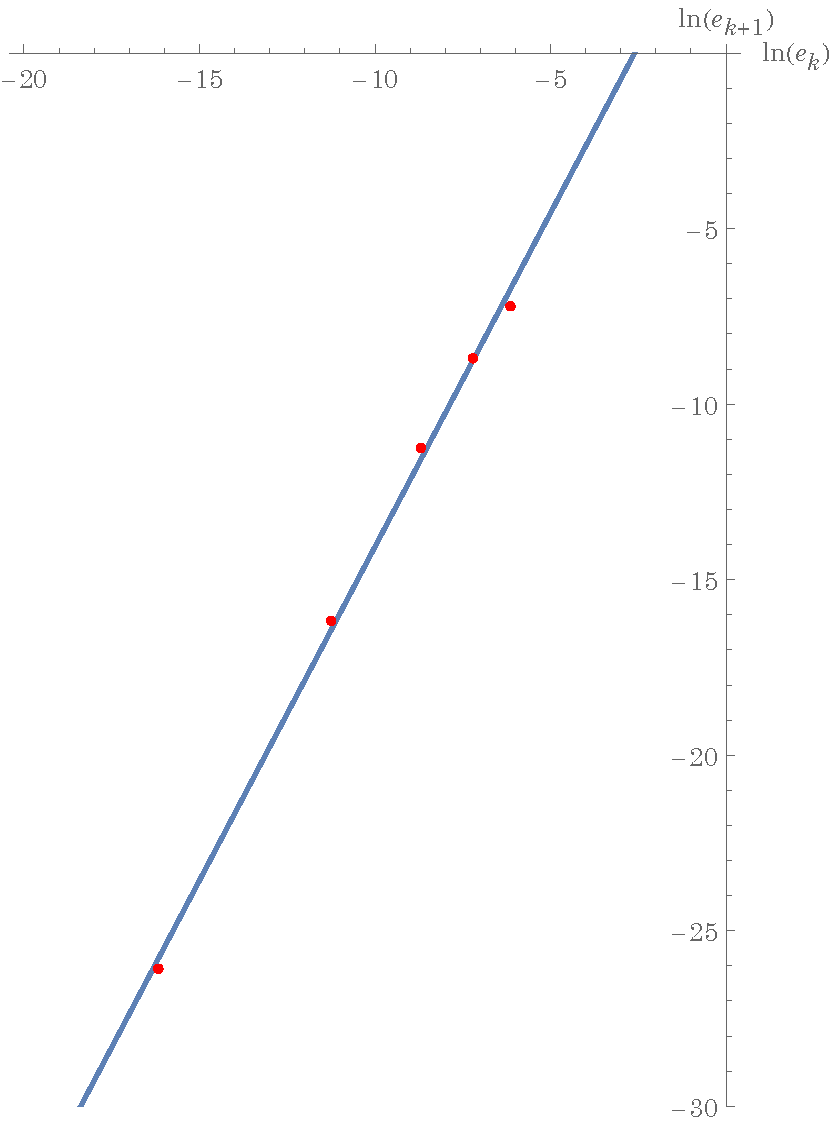
\includegraphics[scale = 0.5]{Figure/收敛阶-Newton2.pdf}
        \label{figure:Newton-LS2}
    \end{subfigure}
    \begin{subfigure}{.49\textwidth}
        \centering
        拟合直线方程为
        \begin{equation*}
            1.90145 x+4.95417
        \end{equation*}
    \end{subfigure}
    \caption{最小二乘拟合Newton 法结果 2 收敛阶}
    \label{Newton-LS2}
\end{figure}
由直线斜率得到初值为 $x_0 = 0$ 和 $x_0 = 3$的 Newton 法迭代的拟合收敛阶分别为$1.8499$和$1.9015$,和理论值$2$较为接近,偏差受有限的迭代次数以及拟合方式影响。

弦截法理论上是$\dfrac{\sqrt{5} + 1}{2} \approx 1.618$阶收敛的,同样选取两组弦截法迭代序列最后 5 个数值点进行拟合,拟合结果如图\ref{Secant-LS1}和\ref{Secant-LS2}所示。
\begin{figure}[h]
    \centering
    \begin{subfigure}{\textwidth}
        \centering
        \resizebox{\textwidth}{!}{
            \begin{tabular}{|c|c|c|c|c|}
                \hline
                迭代步数$k$     & $x_k$                         & $e_k$                        & $\ln{e_{k}}$                  & $\ln{e_{k + 1}}$              \\
                \hline $k = 0$  & $+0.0000000000\text{E}{+}000$ & $1.2132034356\text{E}{-}001$ & $-2.1093207643\text{E}{+}000$ & $-9.7106466498\text{E}{-}001$ \\
                \hline $k = 1$  & $+5.0000000000\text{E}{-}001$ & $3.7867965644\text{E}{-}001$ & $-9.7106466498\text{E}{-}001$ & $-1.7748249826\text{E}{+}000$ \\
                \hline $k = 2$  & $-4.8192771084\text{E}{-}002$ & $1.6951311464\text{E}{-}001$ & $-1.7748249826\text{E}{+}000$ & $-1.2724582475\text{E}{+}000$ \\
                \hline $k = 3$  & $-1.5882177241\text{E}{-}001$ & $2.8014211597\text{E}{-}001$ & $-1.2724582475\text{E}{+}000$ & $-2.2947023711\text{E}{+}000$ \\
                \hline $k = 4$  & $+2.0528956326\text{E}{-}002$ & $1.0079138723\text{E}{-}001$ & $-2.2947023711\text{E}{+}000$ & $-2.6364333585\text{E}{+}000$ \\
                \hline $k = 5$  & $+4.9704099508\text{E}{-}002$ & $7.1616244052\text{E}{-}002$ & $-2.6364333585\text{E}{+}000$ & $-3.1996292671\text{E}{+}000$ \\
                \hline $k = 6$  & $+8.0543024888\text{E}{-}002$ & $4.0777318671\text{E}{-}002$ & $-3.1996292671\text{E}{+}000$ & $-3.6761114026\text{E}{+}000$ \\
                \hline $k = 7$  & $+9.5999095782\text{E}{-}002$ & $2.5321247778\text{E}{-}002$ & $-3.6761114026\text{E}{+}000$ & $-4.1919489838\text{E}{+}000$ \\
                \hline $k = 8$  & $+1.0620354980\text{E}{-}001$ & $1.5116793758\text{E}{-}002$ & $-4.1919489838\text{E}{+}000$ & $-4.7071902948\text{E}{+}000$ \\
                \hline $k = 9$  & $+1.1229022963\text{E}{-}001$ & $9.0301139304\text{E}{-}003$ & $-4.7071902948\text{E}{+}000$ & $-5.2494009620\text{E}{+}000$ \\
                \hline $k = 10$ & $+1.1606968076\text{E}{-}001$ & $5.2506628041\text{E}{-}003$ & $-5.2494009620\text{E}{+}000$ & $-5.8272421392\text{E}{+}000$ \\
                \hline $k = 11$ & $+1.1837415259\text{E}{-}001$ & $2.9461909709\text{E}{-}003$ & $-5.8272421392\text{E}{+}000$ & $-6.4708782413\text{E}{+}000$ \\
                \hline $k = 12$ & $+1.1977247782\text{E}{-}001$ & $1.5478657362\text{E}{-}003$ & $-6.4708782413\text{E}{+}000$ & $-7.2285276758\text{E}{+}000$ \\
                \hline $k = 13$ & $+1.2059475518\text{E}{-}001$ & $7.2558837846\text{E}{-}004$ & $-7.2285276758\text{E}{+}000$ & $-8.1932590634\text{E}{+}000$ \\
                \hline $k = 14$ & $+1.2104383231\text{E}{-}001$ & $2.7651124648\text{E}{-}004$ & $-8.1932590634\text{E}{+}000$ & $-9.5397975729\text{E}{+}000$ \\
                \hline $k = 15$ & $+1.2124841215\text{E}{-}001$ & $7.1931407049\text{E}{-}005$ & $-9.5397975729\text{E}{+}000$ & $-1.1583811433\text{E}{+}001$ \\
                \hline $k = 16$ & $+1.2131102788\text{E}{-}001$ & $9.3156811462\text{E}{-}006$ & $-1.1583811433\text{E}{+}001$ & $-1.4840572041\text{E}{+}001$ \\
                \hline $k = 17$ & $+1.2131998479\text{E}{-}001$ & $3.5877440603\text{E}{-}007$ & $-1.4840572041\text{E}{+}001$ & $-2.0102246753\text{E}{+}001$ \\
                \hline $k = 18$ & $+1.2132034170\text{E}{-}001$ & $1.8608234120\text{E}{-}009$ & $-2.0102246753\text{E}{+}001$ &                               \\
                \hline
            \end{tabular}
        }
        \label{table:Secant-LS1}
    \end{subfigure}
    \begin{subfigure}{.49\textwidth}
        \centering
        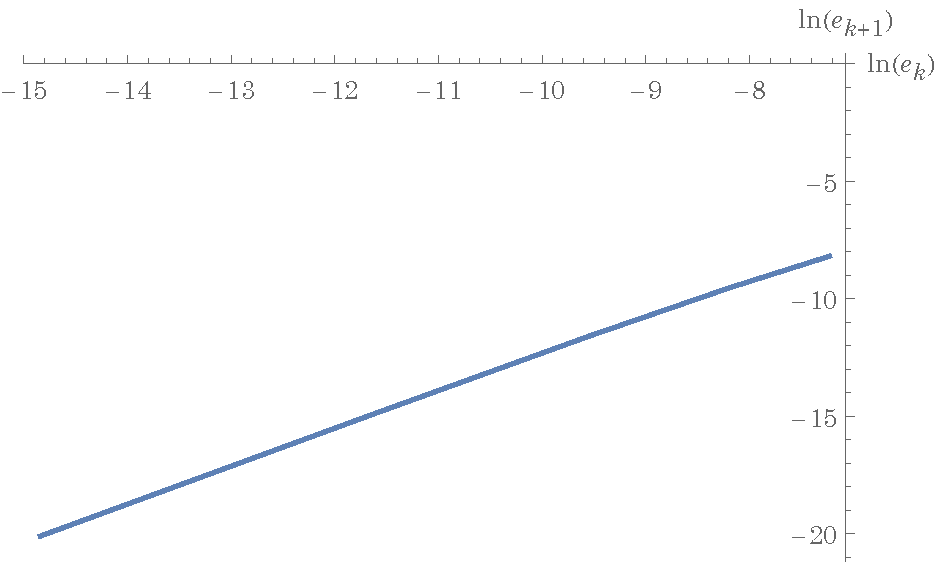
\includegraphics[scale = 0.45]{Figure/收敛阶-Secant1.pdf}
        \label{figure:Secant-LS1}
    \end{subfigure}
    \begin{subfigure}{.49\textwidth}
        \centering
        拟合直线方程为
        \begin{equation*}
            1.57233 x+3.30725
        \end{equation*}
    \end{subfigure}
    \caption{最小二乘拟合弦截法结果 1 收敛阶}
    \label{Secant-LS1}
\end{figure}
\begin{figure}[h]
    \centering
    \begin{subfigure}{\textwidth}
        \centering
        \resizebox{\textwidth}{!}{
            \begin{tabular}{|c|c|c|c|c|}
                \hline
                迭代步数$k$     & $x_k$                        & $e_k$                        & $\ln{e_{k}}$                  & $\ln{e_{k + 1}}$              \\
                \hline $k = 0$  & $1.0000000000\text{E}{-}001$ & $2.1320343560\text{E}{-}002$ & $-3.8480935654\text{E}{+}000$ & $+3.2112627048\text{E}{-}001$ \\
                \hline $k = 1$  & $1.5000000000\text{E}{+}000$ & $1.3786796564\text{E}{+}000$ & $+3.2112627048\text{E}{-}001$ & $-3.8372162786\text{E}{+}000$ \\
                \hline $k = 2$  & $9.9766826661\text{E}{-}002$ & $2.1553516899\text{E}{-}002$ & $-3.8372162786\text{E}{+}000$ & $-3.8262288785\text{E}{+}000$ \\
                \hline $k = 3$  & $9.9528703766\text{E}{-}002$ & $2.1791639793\text{E}{-}002$ & $-3.8262288785\text{E}{+}000$ & $-4.5696455654\text{E}{+}000$ \\
                \hline $k = 4$  & $1.1095871197\text{E}{-}001$ & $1.0361631587\text{E}{-}002$ & $-4.5696455654\text{E}{+}000$ & $-5.0157076803\text{E}{+}000$ \\
                \hline $k = 5$  & $1.1468740718\text{E}{-}001$ & $6.6329363778\text{E}{-}003$ & $-5.0157076803\text{E}{+}000$ & $-5.6123348177\text{E}{+}000$ \\
                \hline $k = 6$  & $1.1766781216\text{E}{-}001$ & $3.6525313994\text{E}{-}003$ & $-5.6123348177\text{E}{+}000$ & $-6.2124300502\text{E}{+}000$ \\
                \hline $k = 7$  & $1.1931598272\text{E}{-}001$ & $2.0043608439\text{E}{-}003$ & $-6.2124300502\text{E}{+}000$ & $-6.9251628551\text{E}{+}000$ \\
                \hline $k = 8$  & $1.2033760050\text{E}{-}001$ & $9.8274306039\text{E}{-}004$ & $-6.9251628551\text{E}{+}000$ & $-7.7934695372\text{E}{+}000$ \\
                \hline $k = 9$  & $1.2090792407\text{E}{-}001$ & $4.1241949404\text{E}{-}004$ & $-7.7934695372\text{E}{+}000$ & $-8.9685814150\text{E}{+}000$ \\
                \hline $k = 10$ & $1.2119299484\text{E}{-}001$ & $1.2734871906\text{E}{-}004$ & $-8.9685814150\text{E}{+}000$ & $-1.0698683037\text{E}{+}001$ \\
                \hline $k = 11$ & $1.2129776891\text{E}{-}001$ & $2.2574648318\text{E}{-}005$ & $-1.0698683037\text{E}{+}001$ & $-1.3420360757\text{E}{+}001$ \\
                \hline $k = 12$ & $1.2131885895\text{E}{-}001$ & $1.4846065701\text{E}{-}006$ & $-1.3420360757\text{E}{+}001$ & $-1.7804888813\text{E}{+}001$ \\
                \hline $k = 13$ & $1.2132032505\text{E}{-}001$ & $1.8511219807\text{E}{-}008$ & $-1.7804888813\text{E}{+}001$ & $-2.4898614592\text{E}{+}001$ \\
                \hline $k = 14$ & $1.2132034354\text{E}{-}001$ & $1.5369830408\text{E}{-}011$ & $-2.4898614592\text{E}{+}001$ &                               \\
                \hline
            \end{tabular}
        }
        \label{table:Secant-LS2}
    \end{subfigure}
    \begin{subfigure}{.49\textwidth}
        \centering
        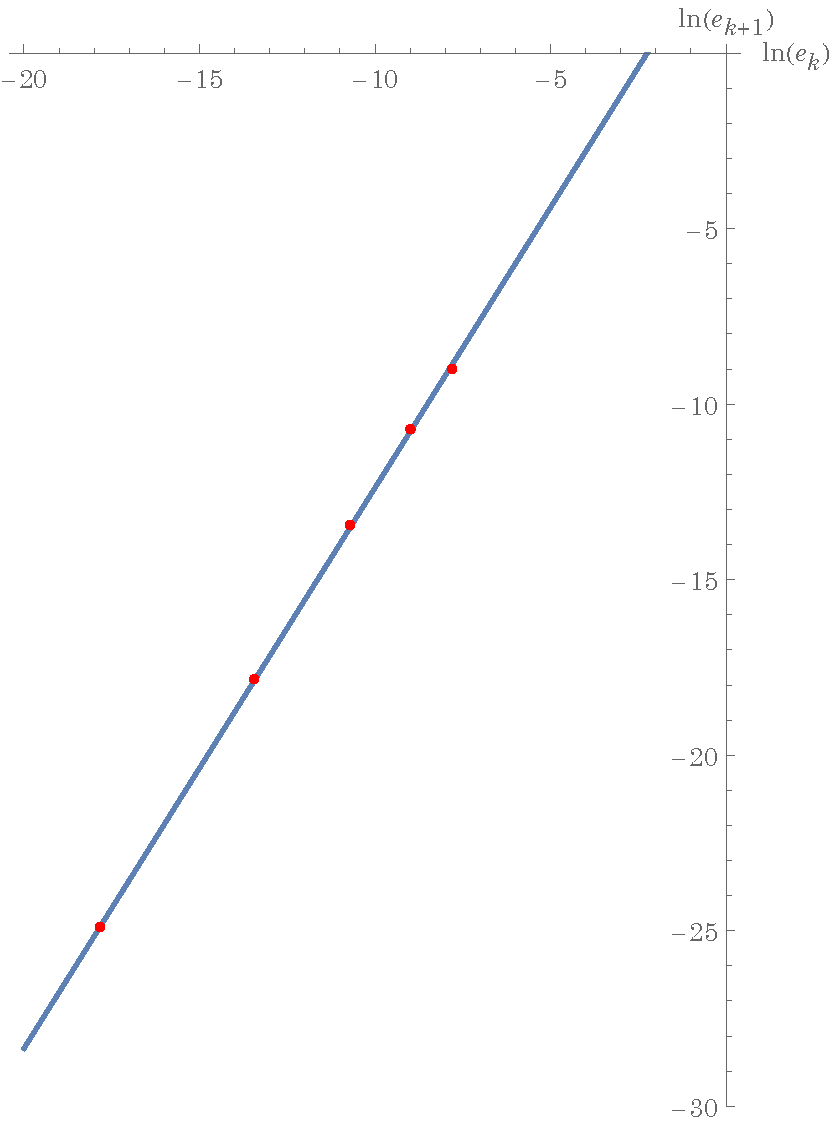
\includegraphics[scale = 0.45]{Figure/收敛阶-Secant2.pdf}
        \label{figure:Secant-LS2}
    \end{subfigure}
    \begin{subfigure}{.49\textwidth}
        \centering
        拟合直线方程为
        \begin{equation*}
            1.59693 x+3.58525
        \end{equation*}
    \end{subfigure}
    \caption{最小二乘拟合弦截法结果 2 收敛阶}
    \label{Secant-LS2}
\end{figure}
由直线斜率得到初值为 $x_0 = 0,\ x_1 = 0.5$ 和 $x_0 = 0.1,\ x_1 = 1.5$弦截法迭代的拟合收敛阶分别为$1.5723$和$1.5969$,和理论值$1.618$也较为接近。

结合四组拟合结果来看,在迭代后期 Newton 法迭代速度确实较弦截法稍快。
\subsection{计算误差}
在算法实现的浮点运算中,会出现舍入误差,对于 Newton 法迭代格式
\begin{equation}
    x_{k + 1} = x_k - \frac{f(x_k)}{f'(x_k)} \tag{6}
\end{equation}
和弦截法迭代格式
\begin{equation*}
    x_{k + 1} = x_k - \frac{f(x_k)(x_k - x_{k - 1})}{f(x_k) - f(x_{k - 1})} \tag{1}
\end{equation*}
Newton 迭代法每次需要计算一次函数值和一次导数值,对于如本次实验中$f(x)$一般的多项式函数,可以机器地得到其导函数并直接进行计算,但对于其他形式的函数,在无法使用符号计算系统得到其导函数或者其导函数形式包含了大量进一步浮点计算步骤时,使用 Newton 法可能引入不可控的计算误差。

而弦截法次只需计算一次函数值,但计算中显式地出现了$x_k - x_{k - 1}$和$f(x_k) - f(x_{k - 1})$,且后者作为分母。当迭代不断进行,这两者的数值都会很小,可能带来更大的舍入误差。

\section{实验结论}
本次实验通过不同初值的两种非线性方程的迭代求解方法—— Newton 法和弦截法对同一个多项式方程进行了数值求解,并对结果进行了比较和分析。在导数值较易得到时 Newton 迭代法有着较为简单的计算过程和更快的迭代速度,而弦截法尽管迭代速度稍慢,但只需要计算一次函数值即可进行迭代,有着更广泛的适用性。

\bibliographystyle{plain}
\bibliography{reference}
\end{document}






